% \VignetteIndexEntry{Bradley-Terry models in R}
% \VignetteKeyword{generalized linear model}
% \VignetteKeyword{logistic regression}
% \VignetteKeyword{penalized quasi-likelihood}
% \VignetteKeyword{ranking}
% \VignetteKeyword{tournament analysis}
% \VignetteKeyword{working residuals}
% \VignettePackage{BradleyTerry2}

%%% For jss:
%% \newcommand{\pkginfo}{}

%%% uncomment for vignette version
\newcommand{\pkginfo}{\small \\[12pt]For \pkg{BradleyTerry2} version \Sexpr{packageDescription("BradleyTerry2")[["Version"]]}, \Sexpr{Sys.Date()}\\\url{https://github.com/hturner/BradleyTerry2}\\[-12pt]}



\setkeys{Gin}{width=0.6\textwidth}

\Rcodeplaceholder{}

%http://www.stat.auckland.ac.nz/~ihaka/downloads/Sweave-customisation.pdf

\newcommand{\R}{\proglang{R}}
\newcommand{\BT}{\pkg{BradleyTerry2}}
\newcommand{\logit}{\mathop{\rm logit}}
\newcommand{\pr}{\mathop{\rm pr}}
\newcommand{\And}{\\}

\author{Heather Turner\\University of Warwick \And
  David Firth\\University of Warwick}
\Plainauthor{Heather Turner, David Firth}

\title{Bradley-Terry Models in \proglang{R}: The \BT\ Package
\pkginfo}
\Plaintitle{Bradley-Terry Models in R: The BradleyTerry2 Package}
\Shorttitle{\pkg{BradleyTerry2}: Bradley-Terry Models in \proglang{R}}

\begin{abstract}
This is a short overview of the \R\ add-on package \BT, which facilitates the
specification and fitting of Bradley-Terry logit, probit or cauchit
models to pair-comparison data.
Included are the standard `unstructured' Bradley-Terry model, structured
versions in which the parameters are related through a linear predictor to
explanatory variables, and the possibility of an order or `home advantage'
effect or other `contest-specific' effects.
Model fitting is either by maximum likelihood, by penalized
quasi-likelihood (for models which involve a random effect), or by bias-reduced
maximum likelihood in which the first-order asymptotic bias of parameter
estimates is eliminated.  Also  provided are a simple and efficient approach to
handling missing covariate data, and suitably-defined residuals for diagnostic
checking of the linear predictor.
\end{abstract}

\Keywords{generalized linear model, logistic regression, penalized quasi-likelihood, ranking, tournament analysis, working residuals}

\Address{
  David Firth\\
  Department of Statistics\\
  University of Warwick\\
  Coventry\\
  CV4 7AL, United Kingdom\\
  E-mail: \email{d.firth@warwick.ac.uk}\\
  URL: \url{http://go.warwick.ac.uk/dfirth}
}


@

\Rcodeplaceholder{}

 %def

\section{Introduction}

The Bradley-Terry model \citep{brad:terr:52} assumes that in a `contest' between
any two `players', say player $i$ and player $j$ $(i, j \in \{1,\ldots,K\})$,
the odds that $i$ beats $j$ are $\alpha_i/\alpha_j$, where $\alpha_i$ and
$\alpha_j$ are positive-valued parameters which might be thought of as
representing `ability'.  A general introduction can be found in
\citet{brad:84} or \citet{agre:02}.
Applications are many, ranging from experimental psychology to the analysis of
sports tournaments to genetics (for example, the allelic
transmission/disequilibrium test of \citealp{sham:curt:95} is based on a
Bradley-Terry model in which the `players' are alleles).
In typical
psychometric applications the `contests' are comparisons, made by
different human subjects, between pairs of items.

% This quicksort algorithm is extracted from Chapter 7, Introduction to Algorithms (3rd edition)
\begin{algorithm}
\caption{Quicksort}
\begin{algorithmic}
\PROCEDURE{Quicksort}{$A, p, r$}
    \IF{$p < r$} 
        \STATE $q = $ \CALL{Partition}{$A, p, r$}
        \STATE \CALL{Quicksort}{$A, p, q - 1$}
        \STATE \CALL{Quicksort}{$A, q + 1, r$}
    \ENDIF
\ENDPROCEDURE
\PROCEDURE{Partition}{$A, p, r$}
    \STATE $x = A[r]$
    \STATE $i = p - 1$
    \FOR{$j = p$ \TO $r - 1$}
        \IF{$A[j] < x$}
            \STATE $i = i + 1$
            \STATE exchange
            $A[i]$ with $A[j]$
        \ENDIF
        \STATE exchange $A[i]$ with $A[r]$
    \ENDFOR
\ENDPROCEDURE
\end{algorithmic}
\end{algorithm}

Try ref ~\ref{sec:BTmodel}

The model can
alternatively be expressed in the logit-linear form
\begin{equation}
\logit[\pr(i\ \mathrm{beats}\ j)]=\lambda_i-\lambda_j,
\label{eq:unstructured}
\end{equation}
where $\lambda_i=\log\alpha_i$ for all $i$.  Thus, assuming independence of all
contests, the parameters $\{\lambda_i\}$ can be estimated by
maximum likelihood using standard software for generalized linear models, with a
suitably specified model matrix.  The primary purpose of the \BT\ package \citep{turn:12},
implemented in the \R\ statistical computing environment \citep{ihak:gent:96,
R}, is to facilitate the specification and fitting of such models and some
extensions.

The \BT\ package supersedes the earlier \pkg{BradleyTerry} package
\citep{firt:05}, providing a more flexible user interface to allow a wider
range of models to be fitted. In particular, \BT\ allows the inclusion of
simple random effects so that the ability parameters can be related to available
explanatory variables through a linear predictor of the form
\begin{equation}
    \lambda_i=\sum_{r=1}^p\beta_rx_{ir} + U_i.
\end{equation}
The inclusion of the prediction
error $U_i$ allows for variability between players with equal covariate values
and induces correlation between comparisons with a common player. \BT\ also
allows for general contest-specific effects to be included in the model and
allows the logit link to be replaced, if required, by a different symmetric link
function (probit or cauchit).

The remainder of the paper is organised as follows. Section~\ref{sec:BTmodel}
demonstrates how to use the \pkg{BradleyTerry2} package to fit a standard
(i.e., unstructured) Bradley-Terry model, with a separate ability parameter estimated for each
player, including the use of bias-reduced estimation for such
models.  Section~\ref{sec:covariates} considers variations of the standard
model, including the use of player-specific variables to model ability and
allowing for contest-specific effects such as an order effect or judge
effects. Sections~\ref{sec:ability} and \ref{sec:residuals} explain how to
obtain important information about a fitted model, in particular the
estimates of ability and their standard errors, and player-level
residuals, whilst
Section~\ref{sec:model} notes the functions available to aid model
search. Section~\ref{sec:data} explains in more detail how set up data for use
with the \BT\ package, Section~\ref{sec:functions} lists the functions
provided by the package and finally Section~\ref{sec:finalremarks}
comments on two directions for further development of the software.

\section{Standard Bradley-Terry model}
\label{sec:BTmodel}

\subsection{Example: Analysis of journal citations}
\label{citations}

The following data come from page 448 of \citet{agre:02}, extracted from the larger
table of \citet{stig:94}.  The data are counts of citations among four prominent
journals of statistics and are included the \BT\ package as the data set
\code{citations}:

\Rcodeplaceholder{}

\Rcodeplaceholder{}

\Rcodeplaceholder{}

 %def
Thus, for example, \emph{Biometrika} was cited 498 times by papers in
\emph{Journal of the American Statistical Association} (JASA) during the period under study.  In order to fit a Bradley-Terry
model to these data using \code{BTm} from the \BT\ package, the data must
first be converted to binomial frequencies. That is, the data need to be
organised into pairs (\code{player1}, \code{player2}) and corresponding
frequencies of wins and losses for \code{player1} against
\code{player2}. The \BT\ package provides the utility function
\code{countsToBinomial} to convert a contingency table of
wins to the format just described:

\Rcodeplaceholder{}

 %def
Note that the self-citation counts are ignored -- these provide no
information on the ability parameters, since the abilities are relative rather than
absolute quantities.
The binomial response can then be modelled by the difference in player abilities
as follows:

\Rcodeplaceholder{}

 %def
The coefficients here are maximum likelihood estimates of $\lambda_2, \lambda_3,
\lambda_4$, with $\lambda_1$ (the log-ability for \emph{Biometrika}) set to zero
as an identifying convention.

The one-sided model formula
\begin{verbatim}
  ~ journal
\end{verbatim}
specifies the model for player ability, in this case the `citeability' of the
journal. The \code{id} argument specifies that \code{"journal"} is the
name to be used for the factor that identifies the player -- the values of which
are given here by \code{journal1} and \code{journal2} for the first and
second players respectively. Therefore in this case a separate
citeability parameter is estimated for each journal.

If a different `reference' journal is required, this can be achieved using the
optional \code{refcat} argument: for
example, making use of \code{update} to avoid re-specifying the whole model,

\Rcodeplaceholder{}

 %def
-- the same model in a different parameterization.

The use of the standard Bradley-Terry model for this application might perhaps
seem rather questionable -- for example, citations within a published paper can
hardly be considered independent, and the model discards potentially important
information on self-citation.  \citet{stig:94} provides arguments to defend the
model's use despite such concerns.

\subsection{Bias-reduced estimates}
%\label{sec:bias}

Estimation of the standard Bradley-Terry model in \code{BTm} is by default
computed by maximum likelihood, using an internal call to the
\code{glm} function.  An alternative  is to fit by bias-reduced
maximum likelihood \citep{firt:93}: this requires additionally the
\pkg{brglm}
package \citep{kosm:07}, and is specified by the optional argument \code{br = TRUE}.  The
resultant effect, namely removal of first-order asymptotic bias in
the estimated coefficients, is often quite small.  One notable feature of
bias-reduced fits is that all estimated coefficients and standard errors are
necessarily finite, even in situations of `complete separation' where maximum
likelihood estimates take
infinite values \citep{hein:sche:02}.

For the citation data, the parameter estimates are only very
slightly changed in the bias-reduced fit:

\Rcodeplaceholder{}

 %def
Here the bias of maximum likelihood is small because the binomial
counts are fairly large.  In more sparse arrangements of contests -- that is,
where there is less
or no replication of the contests -- the effect of bias reduction would
typically be more substantial than the insignificant one seen here.

\section{Abilities predicted by explanatory variables}
\label{sec:covariates}

\subsection{`Player-specific' predictor variables}

In some application contexts there may be `player-specific' explanatory
variables available, and it is then natural to consider model simplification of
the form
\begin{equation}
\lambda_i=\sum_{r=1}^p\beta_rx_{ir} + U_i,
\end{equation}
in which ability of each player $i$ is related to explanatory variables
$x_{i1},\ldots,x_{ip}$ through a linear predictor with coefficients
$\beta_1,\ldots,\beta_p$; the $\{U_i\}$ are independent errors.
Dependence of the player abilities on explanatory variables can be specified via the
\code{formula} argument, using the standard \emph{S}-language
model formulae.  The difference in the abilities of player $i$
and player $j$ is modelled by
\begin{equation}
\sum_{r=1}^p\beta_rx_{ir} - \sum_{r=1}^p\beta_rx_{jr} + U_i - U_j,
\label{eq:structured}
\end{equation}
where $U_i \sim N(0, \sigma^2)$ for all $i$. The Bradley-Terry model is then a
generalized linear mixed model, which the \code{BTm} function currently
fits by using the penalized quasi-likelihood algorithm of \citet{bres:93}.

As an illustration, consider the following simple model for the
\code{flatlizards} data, which predicts the fighting ability of Augrabies flat
lizards by body size (snout to vent length):

\Rcodeplaceholder{}

 %def
Here the winner of each fight is compared to the loser, so the outcome is
always 1.  The special name `\code{..}' appears in the formula as the default
identifier for players, in the absence of a user-specified \code{id} argument.
The values of this factor are given by \code{winner} for the winning lizard
and \code{loser} for the losing lizard in each contest. %Since \code{winner}
%and \code{loser} are specific instances of the factor \code{..}, they must
%share the same set of levels (one for each lizard).
%The factors \code{winner}and \code{loser}
These factors are provided in the data frame \code{contests} that is the
first element of the list object \code{flatlizards}. The second element of
\code{flatlizards} is another data frame, \code{predictors}, containing
measurements on the observed lizards, including \code{SVL}, which is the snout
to vent length. Thus \code{SVL[..]} represents the snout to vent length
indexed by lizard (\code{winner} or \code{loser} as appropriate).  Finally a
random intercept for each lizard is included using the bar notation familiar
to users of the \pkg{lme4} package \citep{bate:11}. (Note that a random intercept is the only random effect
structure currently implemented in \pkg{BradleyTerry2}.)

The fitted model is summarized below:

\Rcodeplaceholder{}

 %def
The coefficient of snout to vent length is weakly significant; however, the
standard deviation of the random effect is quite large,
suggesting that this simple model has fairly poor explanatory power.
A more appropriate model is considered in the next section.

\subsection{Missing values}

The contest data may include all possible pairs of players and hence rows of
missing data corresponding to players paired with themselves. Such rows
contribute no information to the Bradley-Terry model and are simply discarded by
\code{BTm}.

Where there are missing values in player-specific \emph{predictor} (or
\emph{explanatory}) variables which appear in the formula, it
will typically be very wasteful to discard all contests involving players for
which some values are missing. Instead, such cases are accommodated by the
inclusion of one or more parameters in the model.  If, for example, player $1$
has one or more of its predictor values $x_{11},\ldots,x_{1p}$ missing, then the
combination of Equations~\ref{eq:unstructured} and \ref{eq:structured} above yields
\begin{equation}
\logit[\pr(1\ \mathrm{beats}\ j)]=\lambda_1 - \left(\sum_{r=1}^p\beta_rx_{jr} + U_j\right),
\end{equation}
for all other players $j$.  This results in the inclusion of a `direct' ability
parameter for each player having missing predictor values, in addition to the
common coefficients $\beta_1,\ldots,\beta_p$ -- an approach which will be
appropriate when the missingness mechanism is unrelated to contest success.  The
same device can be used also to accommodate any user-specified departures from a
structured Bradley-Terry model, whereby some players have their abilities
determined by the linear predictor but others do not.

In the original analysis of the \code{flatlizards} data \citep{whit:06}, the
final model included the first and third principal components
of the spectral reflectance from the throat (representing brightness and UV intensity
respectively) as well as head length and the snout to vent length seen in our
earlier model. The spectroscopy data was missing for two lizards, therefore
the ability of these lizards was estimated directly. The following fits this
model, with the addition of a random intercept as before:

\Rcodeplaceholder{}

 %def
Note that \code{BTm} detects that lizards 96 and 99 have missing
values in the specified predictors and automatically includes separate ability
parameters for these lizards. This model was found to be the single best model
based on the principal components of reflectance and the other predictors
available and indeed the standard deviation of the random intercept is much
reduced, but still highly significant. Allowing for this significant variation
between lizards with the same predictor values produces more realistic (i.e.,
larger) standard errors for the parameters when compared to the original
analysis of \citet{whit:06}.
Although this affects the significance of the morphological
variables, it does not affect the significance of the principal components, so
in this case does not affect the main conclusions of the study.

\subsection{Order effect}
\label{sec:order}

In certain types of application some or all contests have an associated `bias',
related to the order in which items are presented to a judge or with the
location in which a contest takes place, for example.  A natural extension of
the Bradley-Terry model (Equation~\ref{eq:unstructured}) is then
\begin{equation}
\logit[\pr(i\ \mathrm{beats}\ j)]=\lambda_i-\lambda_j + \delta z,
\end{equation}
where $z=1$ if $i$ has the supposed advantage and $z=-1$ if $j$ has it.  (If the
`advantage' is in fact a disadvantage, $\delta$ will be negative.)  The scores
$\lambda_i$ then relate to ability in the absence of any such advantage.

As an example, consider the baseball data given in \citet{agre:02}, page 438:

\Rcodeplaceholder{}

 %def
The data set records the home wins and losses for each baseball team against each
of the 6 other teams in the data set. The \code{head} function is used to
show the first 6 records, which are the Milwaukee home games. We see for
example that Milwaukee played 7 home games against Detroit and won 4 of them.
The `standard' Bradley-Terry model without a home-advantage parameter will be
fitted if no formula is specified in the call to \code{BTm}:

\Rcodeplaceholder{}

 %def
The reference team is Baltimore, estimated to be the weakest of these seven,
with Milwaukee and Detroit the strongest.

In the above, the ability of each team is modelled simply as \code{~ team} where
the values of the factor \code{team} are given by \code{home.team} for the
first team and \code{away.team} for the second team in each game. To
estimate the home-advantage effect, an additional variable is required to
indicate whether the team is at home or not. Therefore data frames
containing both the team factor and this new indicator variable are required
in place of the factors \code{home.team} and \code{away.team} in the call to
\code{BTm}. This is achieved here by over-writing the \code{home.team} and
\code{away.team} factors in the \code{baseball} data frame:

\Rcodeplaceholder{}

 %def
The \code{at.home} variable is needed for both the home team and the
away team, so that it can be differenced as appropriate in the linear
predictor. With the data organised in this way, the ability formula can now be
updated to include the \code{at.home} variable as follows:

\Rcodeplaceholder{}

 %def

\vspace*{-0.3cm}

This reproduces the results given on page 438 of \citet{agre:02}: the home team
has an estimated odds-multiplier of $\exp(0.3023) = 1.35$ in its favour.

\vspace*{-0.2cm}

\subsection{More general (contest-specific) predictors}
\label{sec:CEMS}

The `home advantage' effect is a simple
example of a contest-specific predictor.  Such predictors are necessarily
interactions, between aspects of the contest and (aspects of) the two
`players' involved.

For more elaborate examples of such effects, see \code{?chameleons} and
\code{?CEMS}.  The former includes an `experience' effect, which changes
through time, on the fighting ability of male chameleons.  The latter
illustrates a common situation in psychometric applications of the
Bradley-Terry model, where \emph{subjects} express preference for one of two
\emph{objects} (the `players'), and it is the influence on the results of
subject attributes that is of primary interest.

As an illustration of the way in which such effects are specified, consider
the following model specification taken from the examples in \code{?CEMS},
where data on students' preferences in relation to six European management
schools is analysed.

\vspace*{-0.3cm}

\Rcodeplaceholder{}

 %def
This model reproduces results from Table~8 of \cite{ditt:01} apart
from minor differences due to the different treatment of ties. Here the
outcome is the binomial frequency of preference for \code{school1}
over \code{school2}, with ties counted as half a `win' and half a `loss'. The
formula specifies the model for school `ability' or worth. In this formula,
the default label `\code{..}' represents the school (with values given by
\code{school1} or \code{school2} as appropriate) and \code{student} is a
factor specifying the student that made the comparison. The remaining
variables in the formula use \proglang{R}'s standard indexing mechanism to include
student-specific variables, e.g., \code{WOR}: whether or not the student was in
full-time employment, and school-specific variables, e.g., \code{LAT}: whether
the school was in a `Latin' city. Thus there are three types of variables:
contest-specific (\code{school1}, \code{school2}, \code{student}),
subject-specific (\code{WOR}, \code{DEG}, \ldots) and object-specific
(\code{LAT}, \code{St.Gallen}, \ldots). These three types of variables are
provided in three data frames, contained in the list object \code{CEMS}.

\section{Ability scores}
\label{sec:ability}

The function \code{BTabilities} extracts estimates and standard errors for
the log-ability scores $\lambda_1, \ldots,\lambda_K$.  These will either be
`direct' estimates, in the case of the standard Bradley-Terry model or for
players with one or more missing predictor values, or `model-based' estimates
of the form $\hat\lambda_i=\sum_{r=1}^p\hat\beta_rx_{ir}$ for players whose ability is
predicted by explanatory variables.

As a simple illustration, team ability estimates in the
home-advantage model for the \code{baseball} data are obtained by:

\Rcodeplaceholder{}

 %def
This gives, for each team, the estimated ability when the team
enjoys no home advantage.

Similarly, estimates of the fighting ability of each lizard in the
\code{flatlizards} data under the model based on the principal components
of the spectral reflectance from the throat are obtained as follows:

\Rcodeplaceholder{}

 %def
%
The ability estimates in an unstructured Bradley-Terry model are
particularly well suited to presentation using the device of
\emph{quasi-variances} \citep{firt:04}.  The \pkg{qvcalc}
package \citep[][version 0.8-5 or later]{firt:10} contains a function of the same name
which does the necessary work:
\begin{verbatim}
> library("qvcalc")
> baseball.qv <- qvcalc(BTabilities(baseballModel2))
> plot(baseball.qv,
+      levelNames = c("Bal", "Bos", "Cle", "Det", "Mil", "NY", "Tor"))
\end{verbatim}
%
\begin{figure}[t!]
    \centering
        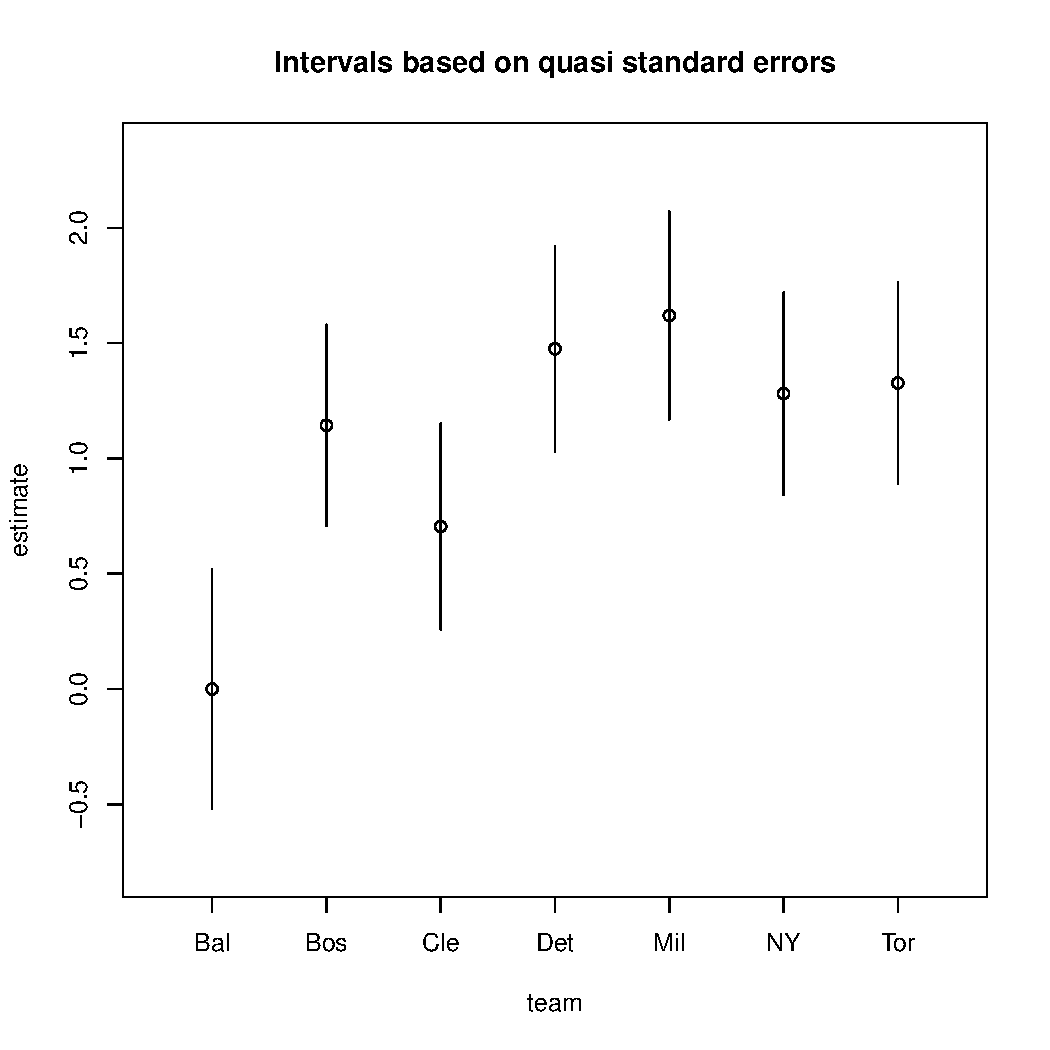
\includegraphics[width=0.67\textwidth]{baseball-qvplot.pdf}
    \caption{Estimated relative abilities of baseball teams.\label{fig:qvplot}}
\end{figure}
%
The `comparison intervals' as shown in Figure~\ref{fig:qvplot} are based on
`quasi standard errors', and can be interpreted as if they refer to
\emph{independent} estimates of ability for the journals.  This has the
advantage that comparison between any pair of journals is readily made
(i.e., not only comparisons with the `reference' journal).  For details
of the theory and method of calculation see \citet{firt:04}.

\section{Residuals}
\label{sec:residuals}

There are two main types of residuals available for a Bradley-Terry model
object.

First, there are residuals obtained by the standard methods for models of class
\code{"glm"}.  These all deliver one residual for each contest or type of
contest.  For example, Pearson residuals for the model
\code{lizModel2} can be obtained simply by

\vspace*{0.2cm}

\Rcodeplaceholder{}

 %def

\vspace*{-0.2cm}

More useful for diagnostics on the linear predictor $\sum\beta_rx_{ir}$ are
`player'-level residuals, obtained by using the function \code{residuals}
with argument \code{type = "grouped"}.  These residuals can then be
plotted against other player-specific variables.

\vspace*{-0.2cm}

\Rcodeplaceholder{}

 %def

\vspace*{-0.2cm}

These residuals estimate the error in the linear predictor; they are obtained by
suitable aggregation of the so-called `working' residuals from the model fit.
The \code{weights} attribute
indicates the relative information in these residuals -- weight is roughly
inversely proportional to variance -- which may be useful for plotting and/or
interpretation; for example, a large residual may be of no real concern if based
on very little information. Weighted least-squares regression of these residuals
on any variable already in the model is null.
For example:

\vspace*{-0.2cm}

\Rcodeplaceholder{}

 %def %$

\vspace*{-0.2cm}

As an illustration of evident \emph{non-null} residual structure, consider the
unrealistically simple model \code{lizModel} that was fitted in
Section~\ref{sec:covariates} above.
That model lacks the
clearly significant predictor variable \code{throat.PC3}, and the
plot shown in Figure~\ref{fig:residuals} demonstrates this fact
graphically:
\begin{verbatim}
> lizModel.residuals <- residuals(lizModel, type = "grouped")
> plot(flatlizards$predictors$throat.PC3, lizModel.residuals)
\end{verbatim}
%
\begin{figure}[t!]
    \centering
        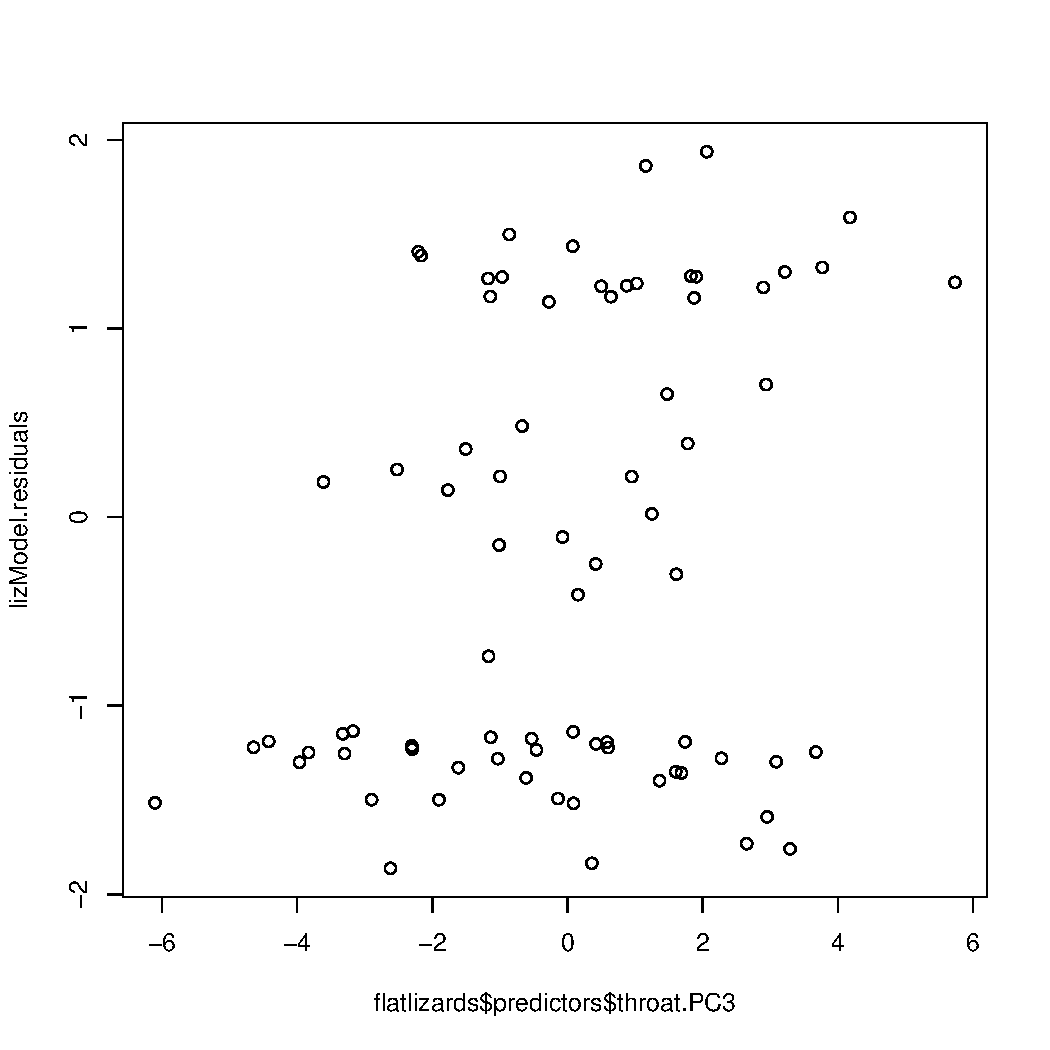
\includegraphics[width=0.69\textwidth]{residuals.pdf}
    \caption{Lizard residuals for the simple model \code{lizModel}, plotted
    against \code{throat.PC3}.\label{fig:residuals}}
\end{figure}
%
The residuals in the plot exhibit a strong, positive regression slope in
relation to the omitted predictor variable \code{throat.PC3}.


\section{Model search}
\label{sec:model}

In addition to \code{update()} as illustrated in preceding sections,
methods for the
generic functions \code{add1()}, \code{drop1()} and
\code{anova()} are provided. These
can be used to investigate the effect of adding or removing a variable, whether
that variable is contest-specific, such as an order effect, or player-specific;
and to compare the fit of nested models.

%These can be used in the standard way for model elaboration or specialization,
%and their availability also allows the use of \texttt{\color{black} step()} for
%automated exploration of a set of candidate player-specific predictors.

\section{Setting up the data}
\label{sec:data}

\subsection{Contest-specific data}
\label{sec:contest}

The \code{outcome} argument of \code{BTm} represents a
binomial response and can be supplied in any of the formats allowed by the
\code{glm} function. That is, either a two-column matrix with the columns
giving the number of wins and losses (for \code{player1} vs.\ \code{player2}),
a factor where the first level denotes a loss and all other levels denote a
win, or a binary variable where 0 denotes a loss and 1 denotes a win. Each row
represents either a single contest or a set of contests between the same two players.

The \code{player1} and \code{player2} arguments are either factors
specifying the two players in each contest, or data frames containing such factors, along
with any contest-specific variables that are also player-specific, such as the
\code{at.home} variable seen in Section~\ref{sec:order}. If given in data
frames, the factors identifying the players should be named as specified by the
\code{id} argument and should have identical levels, since they represent a
particular sample of the full set of players.

Thus for the model \code{baseballModel2}, which was specified by the following call:

\Rcodeplaceholder{}

 %def
the data are provided in the \code{baseball} data frame, which has the
following structure:

\Rcodeplaceholder{}

 %def
In this case \code{home.team} and \code{away.team} are both data frames, with
the factor \code{team} specifying the team and the variable \code{at.home}
specifying whether or not the team was at home. So the first comparison

\Rcodeplaceholder{}

 %def
is Milwaukee playing at home against Detroit. The outcome is given by

\Rcodeplaceholder{}

 %def

Contest-specific variables that are \emph{not} player-specific -- for example,
whether it rained or not during a contest -- should only be used in
interactions with variables that \emph{are} player-specific, otherwise the
effect on ability would be the same for both players and would cancel
out. Such variables can conveniently be provided in a single data frame along with the
\code{outcome}, \code{player1} and \code{player2} data.

An offset in the model can be specified by
using the \code{offset} argument to \code{BTm}\null.  This facility is
provided for completeness: the authors have not yet encountered
an application where it is needed.

To use only certain rows of the contest data in the analysis, the \code{subset}
argument may be used in the call to \code{BTm}.  This should either be a
logical vector of the same length as the binomial response, or a numeric vector
containing the indices of rows to be used.


\subsection{Non contest-specific data}
\label{sec:non-contest}

Some variables do not vary by contest directly, but rather vary by a factor
that is contest-specific, such as the player ID or the judge making the paired
comparison. For such variables, it is more economical to store the data by
the levels of the contest-specific factor and use indexing to obtain the
values for each contest.

The \code{CEMS} example in Section~\ref{sec:CEMS} provides an illustration of
such variables.  In this example student-specific variables are indexed by
\code{student} and school-specific variables are indexed by \code{..}, i.e.,
the first or second school in the comparison as appropriate. There are then
two extra sets of variables in addition to the usual contest-specific data as
described in the last section. A good way to provide these data to \code{BTm}
is as a list of data frames, one for each set of variables, e.g.,

\Rcodeplaceholder{}

 %def
The names of the data frames are only used by \code{BTm} if they match the
names specified in the \code{player1} and \code{player2} arguments, in which
case it is assumed that these are data frames providing the data for the first
and second player respectively. The rows of data frames in the list should
either correspond to the contests or the levels of the factor used for
indexing.

Player-specific offsets should be included in the formula by using the
\code{offset} function.

\subsection{Converting data from a `wide' format}

The \code{BTm} function requires data in a `long' format, with one row per
contest, provided either directly as in Section~\ref{sec:contest} or via
indexing as in Section~\ref{sec:non-contest}. In studies where the same set of
paired comparisons are made by several judges, as in a questionnaire for
example, the data may be stored in a `wide' format, with one row per judge.

As an example, consider the \code{cemspc} data from the \pkg{prefmod} package \citep{hatz:12},
which provides data from the CEMS study in a wide format. Each row corresponds to
one student; the first 15 columns give the outcome of all pairwise comparisons
between the 6~schools in the study and the last two columns correspond to two
of the student-specific variables: \code{ENG} (indicating the student's knowledge
of English) and \code{SEX} (indicating the student's gender).

The following steps convert these data into a form suitable for analysis with
\code{BTm}. First a new data frame is created from the student-specific
variables and these variables are converted to factors:

\Rcodeplaceholder{}

 %def
This data frame is put into a list, which will eventually hold all the
necessary data. Then a \code{student} factor is created for indexing
the student data to produce contest-level data. This is put in a new data frame
that will hold the contest-specific data.

\Rcodeplaceholder{}

 %def
Next the outcome data is converted to a binomial response, adjusted for
ties. The result is added to the \code{contest} data frame.

\Rcodeplaceholder{}

 %def
Then two factors are created identifying the first and second school in each
comparison. The comparisons are in the order 1 vs.\ 2, 1 vs.\ 3, 2 vs.\ 3, 1
vs.\ 4, \ldots, so the factors can be created as follows:

\Rcodeplaceholder{}

 %def
Note that both factors have exactly the same levels, even though only five of
the six players are represented in each case. In other words, the numeric
factor levels refer to the same players in each case, so that the player is
unambiguously identified. This ensures that player-specific parameters and
player-specific covariates are correctly specified.

Finally the \code{contest} data frame is added to the main list:

\Rcodeplaceholder{}

 %def
This creates a single data object that can be passed to the \code{data}
argument of \code{BTm}. Of course, such a list could be created on-the-fly as
in \code{data = list(contest, student)}, which may be more convenient in
practice.

\subsection[Converting data from the format required by the earlier BradleyTerry package]{Converting data from the format required by the earlier \pkg{BradleyTerry} package}

The \pkg{BradleyTerry} package described in \citet{firt:05} required contest/comparison results to be in a data frame with columns named \code{winner}, \code{loser} and \code{Freq}.  The following example shows how \code{xtabs} and \code{countsToBinomial} can be used to convert such data for use with the \code{BTm} function in \pkg{BradleyTerry2}:
\begin{verbatim}
> library("BradleyTerry")  ## the /old/ BradleyTerry package
> ## load data frame with columns "winner", "loser", "Freq"
> data("citations", package = "BradleyTerry")
> ## convert to 2-way table of counts
> citations <- xtabs(Freq ~ winner + loser, citations)
> ## convert to a data frame of binomial observations
> citations.sf <- countsToBinomial(citations)
\end{verbatim}
The \code{citations.sf} data frame can then be used with \code{BTm} as shown in Section~\ref{citations}.



\section[A list of the functions provided in BradleyTerry2]{A list of the functions provided in \pkg{BradleyTerry2}}
\label{sec:functions}

The standard \R\ help files provide the definitive reference.  Here we simply
list the main user-level functions and their arguments, as a
convenient overview:

\Rcodeplaceholder{}

 %def

\section{Some final remarks}
\label{sec:finalremarks}

\subsection[A note on the treatment of ties]{A note on the treatment of ties}

The present version of \BT\ provides no sophisticated facilities for handling
tied contests/comparisons; the well-known models of \cite{rao:kupp:67}
and \cite{davi:70} are not implemented here.  At present the \code{BTm}
function requires a binary or binomial response variable, the third (`tied')
category of response is not allowed.

In several of the data examples (e.g., \code{?CEMS}, \code{?springall},
\code{?sound.fields}),
ties are handled by the crude but simple device of adding half of a `win' to
the tally for each player involved;
in each of the examples where this has been done it is found that the
result is very similar, after a simple re-scaling, to the more
sophisticated analyses that have appeared in the literature.  Note that this
device when used with \code{BTm} typically gives rise to warnings
produced by the back-end
\code{glm} function, about non-integer `binomial' counts; such warnings
are of no consequence and can be safely ignored.

It is likely that a future version of \BT\ will have a more general
method for handling ties.

\subsection{A note on `contest-specific' random effects}

The current version of \BT\ provides facilities for fitting models with
random effects in `player-specific' predictor functions, as illustrated
in Section~\ref{sec:covariates}.
For more general, `contest-specific' random-effect structures,
such as random `judge'
effects in psychological studies \citep[e.g.,][]{bock:01}, \BT\ provides
(through \code{BTm}) the necessary user interface but as yet no
back-end calculation.  It is hoped that this important generalization
can be made successfully in a future version of \BT.

\section*{Acknowledgments}

This work was supported by the UK Engineering and Physical Sciences Research
Council.


\begin{thebibliography}{22}
\newcommand{\enquote}[1]{``#1''}
\providecommand{\natexlab}[1]{#1}
\providecommand{\url}[1]{\texttt{#1}}
\providecommand{\urlprefix}{URL }
\expandafter\ifx\csname urlstyle\endcsname\relax
  \providecommand{\doi}[1]{doi:\discretionary{}{}{}#1}\else
  \providecommand{\doi}{doi:\discretionary{}{}{}\begingroup
  \urlstyle{rm}\Url}\fi
\providecommand{\eprint}[2][]{\url{#2}}

\bibitem[{Agresti(2002)}]{agre:02}
Agresti A (2002).
\newblock \emph{Categorical Data Analysis}.
\newblock 2nd edition. John Wiley \& Sons.

\bibitem[{Bates \emph{et~al.}(2011)Bates, M\"achler, and Bolker}]{bate:11}
Bates D, M\"achler M, Bolker B (2011).
\newblock \emph{\pkg{lme4}: Linear Mixed-Effects Models Using \proglang{S}4
  Classes}.
\newblock \proglang{R}~package version~0.999375-42,
  \urlprefix\url{http://CRAN.R-project.org/package=lme4}.

\bibitem[{B\"ockenholt(2001)}]{bock:01}
B\"ockenholt U (2001).
\newblock \enquote{Hierarchical Modeling of Paired Comparison Data.}
\newblock \emph{Psychological Methods}, \textbf{6}(1), 49--66.

\bibitem[{Bradley(1984)}]{brad:84}
Bradley RA (1984).
\newblock \enquote{Paired Comparisons: Some Basic Procedures and Examples.}
\newblock In PR~Krishnaiah, PK~Sen (eds.), \emph{Nonparametric Methods},
  volume~4 of \emph{Handbook of Statistics}, pp. 299 -- 326. Elsevier.

\bibitem[{Bradley and Terry(1952)}]{brad:terr:52}
Bradley RA, Terry ME (1952).
\newblock \enquote{Rank Analysis of Incomplete Block Designs {I}: {T}he Method
  of Paired Comparisons.}
\newblock \emph{Biometrika}, \textbf{39}, 324--45.

\bibitem[{Breslow and Clayton(1993)}]{bres:93}
Breslow NE, Clayton DG (1993).
\newblock \enquote{Approximate Inference in Generalized Linear Mixed Models.}
\newblock \emph{Journal of the American Statistical Association},
  \textbf{88}(421), 9--25.

\bibitem[{Davidson(1970)}]{davi:70}
Davidson RR (1970).
\newblock \enquote{On Extending the {B}radley-{T}erry Model to Accommodate Ties
  in Paired Comparison Experiments.}
\newblock \emph{Journal of the American Statistical Association}, \textbf{65},
  317--328.

\bibitem[{Dittrich \emph{et~al.}(2001)Dittrich, Hatzinger, and
  Katzenbeisser}]{ditt:01}
Dittrich R, Hatzinger R, Katzenbeisser W (2001).
\newblock \enquote{Corrigendum: {M}odelling the Effect of Subject-Specific
  Covariates in Paired Comparison Studies with an Application to University
  Rankings.}
\newblock \emph{Applied Statistics}, \textbf{50}, 247--249.

\bibitem[{Firth(1993)}]{firt:93}
Firth D (1993).
\newblock \enquote{Bias Reduction of Maximum Likelihood Estimates.}
\newblock \emph{Biometrika}, \textbf{80}, 27--38.

\bibitem[{Firth(2005)}]{firt:05}
Firth D (2005).
\newblock \enquote{Bradley-Terry Models in \proglang{R}.}
\newblock \emph{Journal of Statistical Software}, \textbf{12}(1), 1--12.
\newblock \urlprefix\url{http://www.jstatsoft.org/v12/i01/}.

\bibitem[{Firth(2010)}]{firt:10}
Firth D (2010).
\newblock \emph{\pkg{qvcalc}: Quasi-Variances for Factor Effects in Statistical
  Models}.
\newblock \proglang{R}~package version~0.8-7,
  \urlprefix\url{http://CRAN.R-project.org/package=qvcalc}.

\bibitem[{Firth and {de Menezes}(2004)}]{firt:04}
Firth D, {de Menezes} RX (2004).
\newblock \enquote{Quasi-Variances.}
\newblock \emph{Biometrika}, \textbf{91}, 65--80.

\bibitem[{Hatzinger and Dittrich(2012)}]{hatz:12}
Hatzinger R, Dittrich R (2012).
\newblock \enquote{\pkg{prefmod}: An \proglang{R} Package for Modeling
  Preferences Based on Paired Comparisons, Rankings, or Ratings.}
\newblock \emph{Journal of Statistical Software}, \textbf{48}(10), 1--31.
\newblock \urlprefix\url{http://www.jstatsoft.org/v48/i10/}.

\bibitem[{Heinze and Schemper(2002)}]{hein:sche:02}
Heinze G, Schemper M (2002).
\newblock \enquote{A Solution to the Problem of Separation in Logistic
  Regression.}
\newblock \emph{Statistics in Medicine}, \textbf{21}, 2409--2419.

\bibitem[{Ihaka and Gentleman(1996)}]{ihak:gent:96}
Ihaka R, Gentleman R (1996).
\newblock \enquote{\proglang{R}: A Language for Data Analysis and Graphics.}
\newblock \emph{Journal of Computational and Graphical Statistics},
  \textbf{5}(3), 299--314.

\bibitem[{Kosmidis(2007)}]{kosm:07}
Kosmidis I (2007).
\newblock \emph{\pkg{brglm}: Bias Reduction in Binary-Response GLMs}.
\newblock \proglang{R}~package version~0.5-6,
  \urlprefix\url{http://www.ucl.ac.uk/~ucakiko/software.html}.

\bibitem[{Rao and Kupper(1967)}]{rao:kupp:67}
Rao PV, Kupper LL (1967).
\newblock \enquote{Ties in Paired-Comparison Experiments: {A} Generalization of
  the {B}radley-{T}erry Model.}
\newblock \emph{Journal of the American Statistical Association}, \textbf{62},
  194--204.

\bibitem[{{\proglang{R} Development Core Team}(2012)}]{R}
{\proglang{R} Development Core Team} (2012).
\newblock \emph{\proglang{R}: A Language and Environment for Statistical
  Computing}.
\newblock \proglang{R} Foundation for Statistical Computing, Vienna, Austria.
\newblock {ISBN} 3-900051-07-0, \urlprefix\url{http://www.R-project.org/}.

\bibitem[{Sham and Curtis(1995)}]{sham:curt:95}
Sham PC, Curtis D (1995).
\newblock \enquote{An Extended Transmission/Disequilibrium Test ({TDT}) for
  Multi-Allele Marker Loci.}
\newblock \emph{Annals of Human Genetics}, \textbf{59}(3), 323--336.

\bibitem[{Stigler(1994)}]{stig:94}
Stigler S (1994).
\newblock \enquote{Citation Patterns in the Journals of Statistics and
  Probability.}
\newblock \emph{Statistical Science}, \textbf{9}, 94--108.

\bibitem[{Turner and Firth(2012)}]{turn:12}
Turner H, Firth D (2012).
\newblock \enquote{Bradley-Terry Models in \proglang{R}: The
  \pkg{BradleyTerry2} Package.}
\newblock \emph{Journal of Statistical Software}, \textbf{48}(9), 1--21.
\newblock \urlprefix\url{http://www.jstatsoft.org/v48/i09/}.

\bibitem[{Whiting \emph{et~al.}({2006})Whiting, Stuart-Fox, O'Connor, Firth,
  Bennett, and Blomberg}]{whit:06}
Whiting MJ, Stuart-Fox DM, O'Connor D, Firth D, Bennett NC, Blomberg SP
  ({2006}).
\newblock \enquote{{Ultraviolet Signals Ultra-Aggression in a Lizard}.}
\newblock \emph{Animal Behaviour}, \textbf{{72}}, 353--363.

\end{thebibliography}


\bibliography{BradleyTerry-generated}
